% ****** Start of file aipsamp.tex ******
%
%   This file is part of the AIP files in the AIP distribution for REVTeX 4.
%   Version 4.1 of REVTeX, October 2009
%
%   Copyright (c) 2009 American Institute of Physics.
%
%   See the AIP README file for restrictions and more information.
%
% TeX'ing this file requires that you have AMS-LaTeX 2.0 installed
% as well as the rest of the prerequisites for REVTeX 4.1
% 
% It also requires running BibTeX. The commands are as follows:
%
%  1)  latex  aipsamp
%  2)  bibtex aipsamp
%  3)  latex  aipsamp
%  4)  latex  aipsamp
%
% Use this file as a source of example code for your aip document.
% Use the file aiptemplate.tex as a template for your document.

\documentclass[aip,rsi,amsmath,amssymb,reprint]{revtex4-1}
%\documentclass[%
% aip,
% jmp,
% bmf,
% sd,
% rsi,
% amsmath,amssymb,
% preprint,%
% reprint,%
%author-year,%
%author-numerical,%
%Conference Proceedings
%]{revtex4-1}

\usepackage{graphicx}% Include figure files
\usepackage{dcolumn}% Align table columns on decimal point
\usepackage{bm}% bold math
%\usepackage[mathlines]{lineno}% Enable numbering of text and display math
%\linenumbers\relax % Commence numbering lines

\usepackage[utf8]{inputenc}
\usepackage[T1]{fontenc}
\usepackage{mathptmx}

\begin{document}

%\preprint{AIP/123-QED}

\title[A simple vacuum suitcase for plasma facing component characterization in fusion devices]{A simple vacuum suitcase for plasma facing component characterization in fusion devices}% Force line breaks with \\
%\thanks{Footnote to title of article.}

\author{A. Maan}
%Lines break automatically or can be forced with \\
 \email{amaan@vols.utk.edu}
\affiliation{ 
University of Tennessee, Knoxville%\\This line break forced with \textbackslash\textbackslash
}% 
 \affiliation{Princeton Plasma Physics Laboratory}
 
\author{R. Kaita}%
\affiliation{Princeton Plasma Physics Laboratory}
\affiliation{ 
University of Tennessee, Knoxville%\\This line break forced with \textbackslash\textbackslash
}%

\author{E.T. Ostrowski}
\affiliation{% 
Princeton University%\\This line break forced% with \\
}%

\author{R. Majeski}
\affiliation{% 
Princeton Plasma Physics Laboratory%\\This line break forced% with \\
}%

\author{D.P. Boyle}
\affiliation{% 
Princeton Plasma Physics Laboratory%\\This line break forced% with \\
}%

\author{D.C. Donovan}
\affiliation{ 
University of Tennessee, Knoxville%\\This line break forced with \textbackslash\textbackslash
}%

\author{R.A. Ellis}
\affiliation{% 
Princeton Plasma Physics Laboratory%\\This line break forced% with \\
}%

\author{B.E. Koel}
\affiliation{% 
Princeton University%\\This line break forced% with \\
}%

\author{T.M. Biewer}
\affiliation{% 
Oak Ridge National Laboratory%\\This line break forced% with \\
}%

\date{\today}% It is always \today, today,
             %  but any date may be explicitly specified

\begin{abstract}
We have demonstrated that a vacuum suitcase (Sample Exposure Probe) can be suitably designed as an in-vacuo sample analysis solution for Plasma Facing Component (PFC) characterization of tokamaks. A similar system could be implemented for other fusion devices. Provided vacuum conditions are an order of magnitude or better during transfer and analysis, the quantity of impurities then introduced during transfer and analysis is lower compared to the impurities introduced by the tokamak residual vacuum conditions for the same time; this enables analysis at more powerful stations that are not encumbered by design constraints imposed on them by a tokamak. The vacuum suitcase is an alternative solution to characterizing PFCs using diagnostics that are designed and built around a tokamak, an example of which is the Material Analysis and Particle Probe (MAPP). MAPP was installed on the Lithium Tokamak eXperiment (LTX), and made key observations regarding oxygen uptake of lithium. Its limitations however, led to the need to design the Sample Exposure Probe (SEP). The SEP features a stainless steel probe head with a button heater to heat the probe head for Temperature Programmed Desorption (TPD) studies and to mimic LTX-$\beta$ (LTX upgrade) shells in high temperature operations, a thermocouple inserted in the back of the sample head to measure heat flux from the plasma during exposure and to monitor the temperature during TPD. 
\end{abstract}

\keywords{Plasma Material Interaction, Vacuum Suitcase, Lithium Plasma Facing Component, X-Ray Photoelectron Spectroscopy, Portable, Ultra-High Vacuum}%Use showkeys class option if keyword
                              %display desired
\maketitle

\section{\label{sec:level1}Introduction}

Low-Z coatings, especially lithium, have improved plasma performance in various machines, including TFTR, NSTX, CDX-U, LTX and EAST \cite{tftr,bob-lucia,cdx,ltx,east}. Lithium coatings on both high $Z$ (stainless steel in CDX-U and LTX) and low $Z$ (graphite in TFTR and NSTX) plasma facing components (PFCs) have produced encouraging results. The original idea behind using lithium (Li) to condition surfaces was to bind hydrogen and its isotopes in an ionic bond (LiH), as occurs in the absence of any oxygen in a non-tokamak environment \cite{doerner}. Such gettering of hydrogen ions from the plasma by lithium provides access to a low recycling regime.

The Materials Analysis and Particle Probe (MAPP) was designed to characterize PFC surfaces in-vacuo, i.e., without any exposure to air. MAPP was used initially on LTX at the Princeton Plasma Physics Laboratory (PPPL), where the samples were inserted to be flush with the plasma facing surfaces of the conducting shells \cite{lucia-paper, lucia-thesis}. Samples on the probe head included those made of stainless steel (SS-304 and SS-316) to match the LTX shells. The LTX shells and samples were then coated with lithium, after which the probe head was exposed to LTX plasma. Post exposure, the probe was retracted in-vacuo into the MAPP analysis chamber for X-Ray Photoelectron Spectroscopy (XPS) determination of the surface composition of the SS-304 MAPP sample. XPS indicated an increase in the oxygen concentration of the sample after exposure to LTX residual vacuum conditions, which was attributed to oxidation by water vapor that was observed by the Residual Gas Analyzer (RGA).

%\begin{figure}%
%\centering
%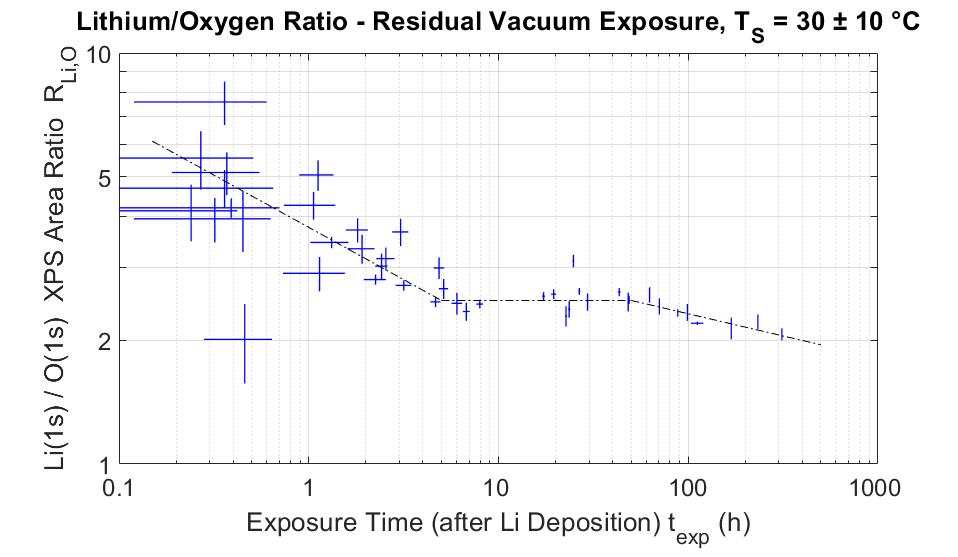
\includegraphics[width=3.37in,keepaspectratio]{Ratio}%
%\caption{Ratio of $Li(1s)$ to $O(1s)$ signal as a function of exposure to LTX %residual vacuum conditions \cite{bob-lucia}}
%\end{figure}

Temporal evolution of lithium and oxygen concentrations were also tracked using MAPP. It was observed that the Li(1s)/O(1s) ratio decreased, until it saturated the XPS probe depth, within 5 hrs \cite{lucia-thesis,lucia-paper}. Beyond that, there was no observable change in the elemental concentration until 100 hrs, after which the Li(1s)/O(1s) ratio began to decrease slowly. The saturation of the ratio of lithium to oxygen to about 2 was attributed to the growth of Li$_2$O on freshly deposited lithium in the presence of residual water vapor, consistent with laboratory experiments \cite{50,51}. Specifically, below 100 Langmuirs (1 L = 10$^{-6}$ Torr-sec) of H$_2$O exposure, Li$_2$O forms preferentially on a clean lithium surface, while at higher exposures there is a transition to LiOH formation. For LTX-relevant water partial pressures, 100 L is equivalent 14 hrs of exposure to residual vacuum. It was also observed that the presence of the oxide did not degrade plasma performance; LTX continued to get high plasma currents until 40 days after lithium deposition\cite{bob-lucia}. 

An explanation of the oxide growth can be provided by the metal oxide growth kinetics model \cite{53}, which states that, in general the oxide growth kinetics can be modelled by an advection-diffusion equation. At the onset, the oxide growth is driven by advection; a potential develops across the oxide film that drives the metal ions to the gas-oxide interface and oxygen ions to the metal-oxide interface. As the oxide grows in thickness, the potential across the film is shielded by free electrons and eventually, when the oxide grows thick enough, further growth is dominated by Fickian diffusion. The flux of H$_2$O molecules impinging onto the surface in LTX after lithium deposition was $\Gamma_{\text{H}_2\text{O}} = 5.6 \times 10^{15} $m$^{-2}$sec$^{-1}$. Assuming a sticking co-efficient\cite{51} S = 1, with this flux it would take 13 min for a monolayer of oxide to form. Since the Li(1s)/O(1s) ratio saturates to $\sim$ 2 after 5 hr \cite{lucia-thesis,lucia-paper}, we assume that the oxide layer took 5 hrs to grow 3 nm in thickness, because 3 nm is the approximate XPS probe depth for MAPP. The metal oxide growth kinetics model then dictates an oxide growth rate of 0.72 nm/hr at the onset and 0.55 nm/hr at the XPS probe depth in the thin film limit \cite{thin-film}. Note that the oxide growth rate would continue to decrease slowly as the film thickness increased. At the oxide growth rate of 5.5 nm/hr, a 100 nm coating would take 180 hr to fully oxidize, which is close to the 100 hr period for which there was no observable change in the Li(1s)/O(1s) ratios. \cite{lucia-thesis,lucia-paper} Therefore, it was concluded that lithium coatings on LTX change over a timescale of hours. 

Immediately after the plasma extinguished in LTX, the Fast Ion Gauge showed a 60\% reduction in H$_2$ inventory compared to calibration gas puffs where a plasma was not initiated \cite{bob-lucia,boyle-prl}. Over longer timescales, however, the H$_2$ reading in the Residual Gas Analyzer (RGA) for shots when a plasma was initiated exceeds the recorded measurement for the calibrated gas puffs. This leads to the conclusion that while a significant portion of hydrogen is retained during a plasma, the hydrogen out-gasses over time scales much longer than the plasma duration \cite{bob-lucia}. With 60\% of the hydrogen fueled in, retained, for a lithium coating of 100 nm and LTX relevant fluence, the Li coating would saturate with hydrogen in $<$ 10 shots (assuming Li:H = 1:1). However, this was not the case and neither H retention nor plasma performance decayed after a few shots, rather after 40 days and close to tens of shots. This leads to the conclusion that hydrogen is retained by lithium coated PFCs in LTX such that it is free to diffuse out between shots. The conclusions regarding the state of the PFC using MAPP results were arrived at using elemental abundances only, in-spite of the fact that binding energy shifts, quantified using XPS can be used to identify chemical states. MAPP did not have the energy resolution to identify different species of Li that grew on the PFCs.

\section{Description of Apparatus}

In the previous campaign, LTX operated with a toroidal field $\sim$ 1.7 kG, I$_p$ $<$ 80 kA and a shot duration $\tau_{discharge}$ $<$ 25 msec.An upgrade to LTX, LTX-$\beta$ can achieve double the field and plasma current and close to double the discharge duration with neutral beam fueling. To further study the effect of lithium PFCs on plasma performance in LTX-$\beta$, we have constructed a Sample Exposure Probe (SEP).

\begin{figure}%
\centering
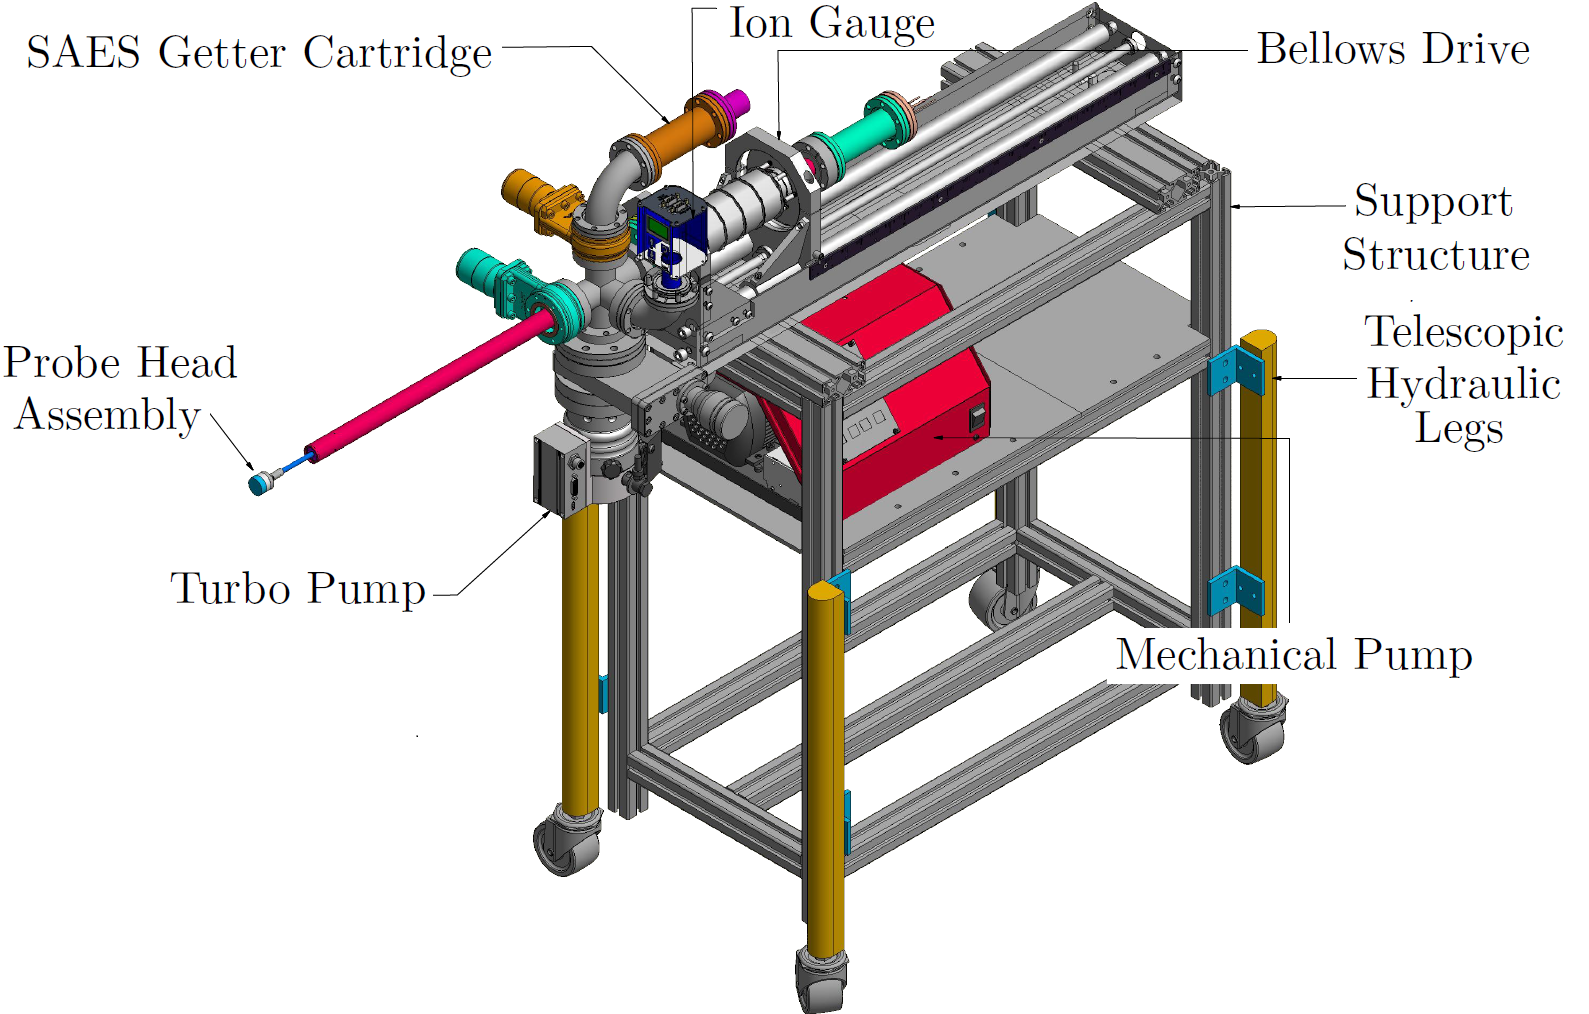
\includegraphics[width=3.37in,keepaspectratio]{SEP_Annotated}%
\caption{Isometric view of the Sample Exposure Probe Assembly}
\end{figure}

The SEP, figure 1, is equipped with a 67 L/sec turbomolecular pump and a 100 L/sec non-evaporable getter pump. The assembly is mounted in a bellows drive and the drive rests on a support structure with telescopic hydraulic legs to facilitate mounting on LTX-$\beta$ and the PHI surface analysis chamber. The PHI is a UHV (Ultra-High Vacuum) chamber in the Surface Science and Technology Laboratory (SS\&TL) near LTX-$\beta$ at PPPL. PHI is equipped for XPS, TPD, Ion Scattering Spectroscopy (ISS) and Sputter Depth Profiling. The PHI has a base pressure of 2 \times $10^{-10}$ Torr; pumping is provided by a 120 L/sec ion pump, a 170 L/sec turbomolecular pump, a 1000 L/sec titanium getter and a 30 L/sec turbomolecular pump for differentially pumping the ion source. The SEP has a base pressure of $1.6 \times 10^{-9}$ Torr; the base pressure of LTX-$\beta$ after lithium evaporation is $6 \times 10^{-8}$ Torr. Therefore, in-vacuo analysis can be performed for LTX-$\beta$ PFCs by moving samples in-vacuo, under better vacuum conditions to a high resolution system that is nearby. In doing so, design constraints that are imposed on the analysis station, for example by the test cell of the tokamak are eliminated, enabling analysis with systems that posses higher resolution and better signal to noise ratios. Better vacuum conditions during transfer and analysis reduce the rate of sample contamination and therefore, provide adequate time required for physical transfer of the probe, its analysis and return to the tokamak. 

\begin{figure}%
\centering
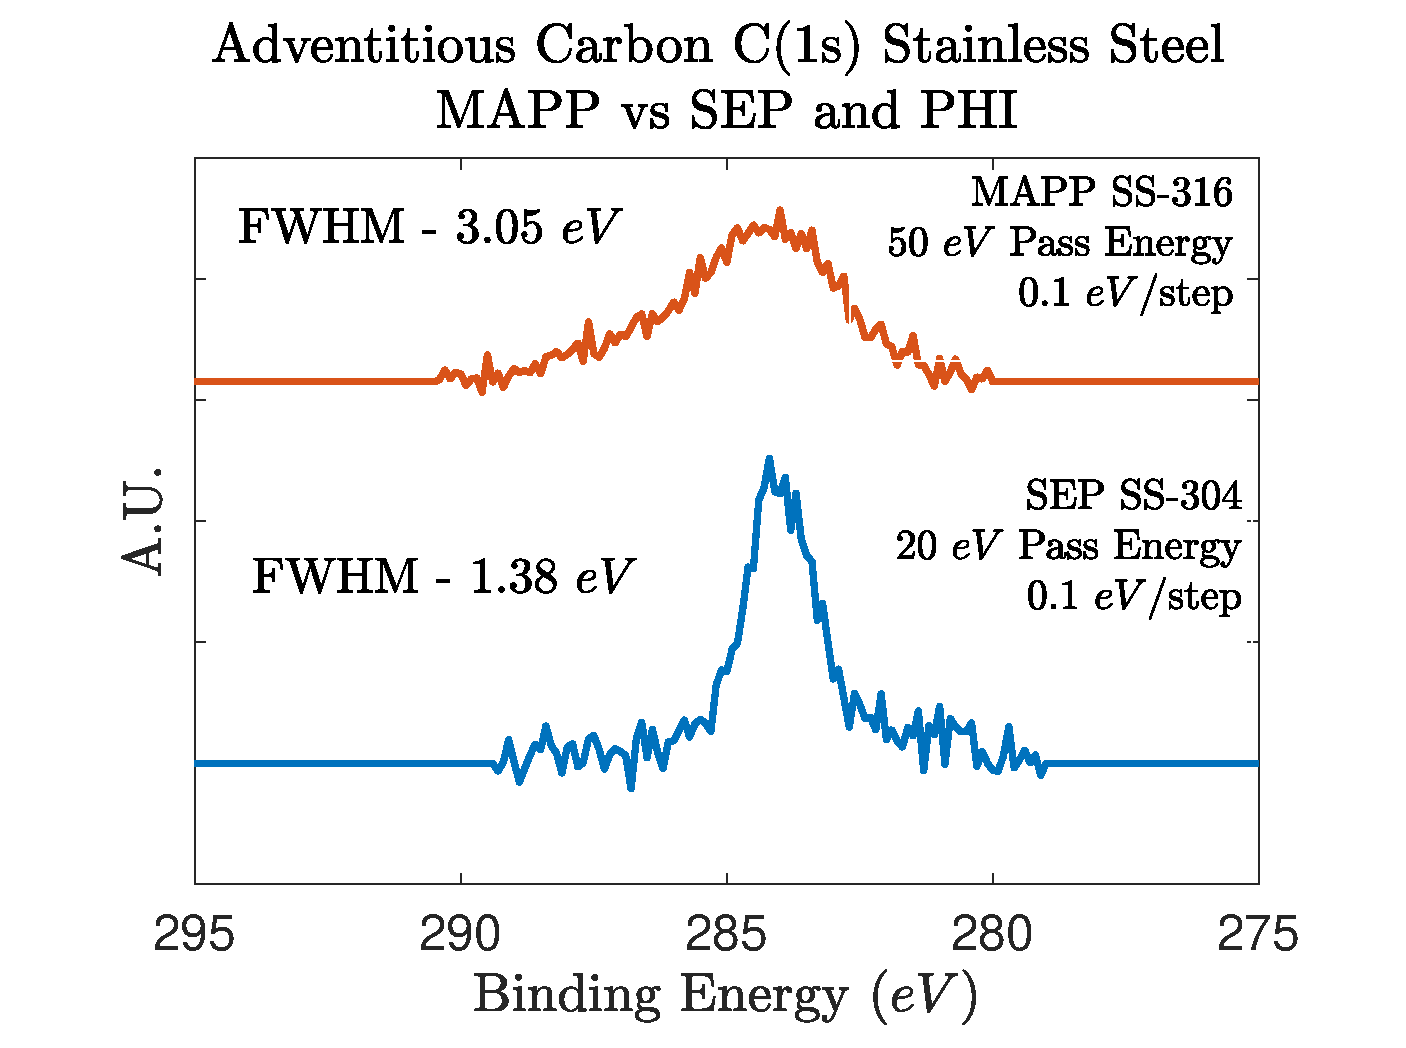
\includegraphics[width=3.37in,keepaspectratio]{C1sMAPP_Comparr_20eV}%
\caption{Adventitious Carbon C(1s) peak on MAPP and SEP}
\end{figure}

\section{Performance and Comparison}

Better resolution and signal to noise ratio (SNR) on XPS scans help understand how surfaces change in a tokamak and consequently in understanding how they impact plasma performance. Initial XPS scans using the SEP on the PHI show both improved resolution and better signal to noise ratio. An example of this improvement is shown in figure 2, the two scans belong to the adventitious carbon $C(1s)$ peak on the stainless steel probe head of MAPP and SEP respectively. The scans show a reduction in full width at half maximum (FWHM) by a factor of 2.2. SNR was measured for both peaks using a commonly used expression for XPS \cite{xps_snr} to be 13.5 for the MAPP peak and 23 for the SEP using PHI. This is because of the higher intensity of the X-Ray source on the PHI and a smaller distance to the probe head. The $C(1s)$ peak shown in figure 2, blue (bottom) trace, at $50 eV$ pass energy shows a FWHM of $1.8eV$ and an SNR of 64. 

\begin{figure}%
\centering
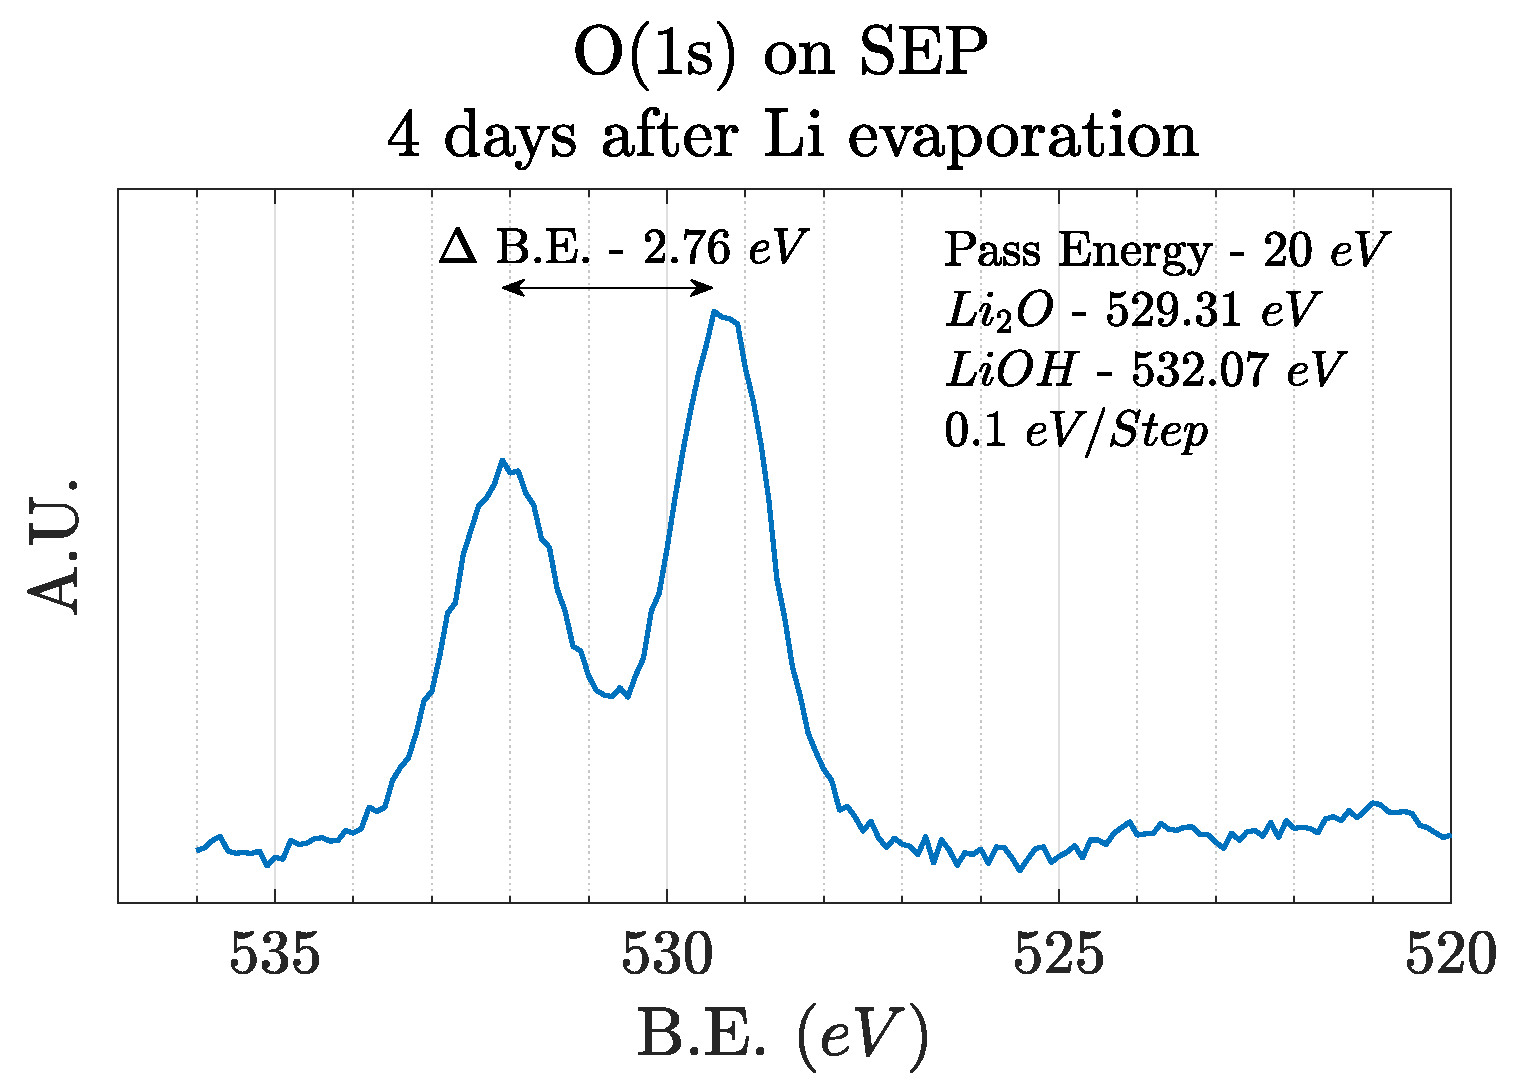
\includegraphics[width=3.37in,keepaspectratio]{O1s_20eV}%
\caption{O(1s) narrow scan of the SEP }
\end{figure}

An example of how improved resolution on XPS scans is helpful in identifying species on the surface is shown in figure 3. It was hypothesized by the previous analysis that LiOH grows on the surface of Li deposited on SS shells of LTX over longer time scales (i.e., hours and beyond), but MAPP did not have the requisite resolution to confirm this. Figure 3 shows a narrow $O(1s)$ scan of the SEP probe head. The scan was taken 4 days after fresh lithium was deposited on the LTX-$\beta$ shells. The SEP was docked on LTX-$\beta$, and the probe head was made flush with the shells during the Li deposition and subsequent plasma and residual vacuum exposure. The narrow $O(1s)$ scans show two distinct features; the difference in binding energy of the two features is consistent with the reported difference between Li$_2$O and LiOH \cite{o1s_delta}. 

\begin{figure}%
\centering
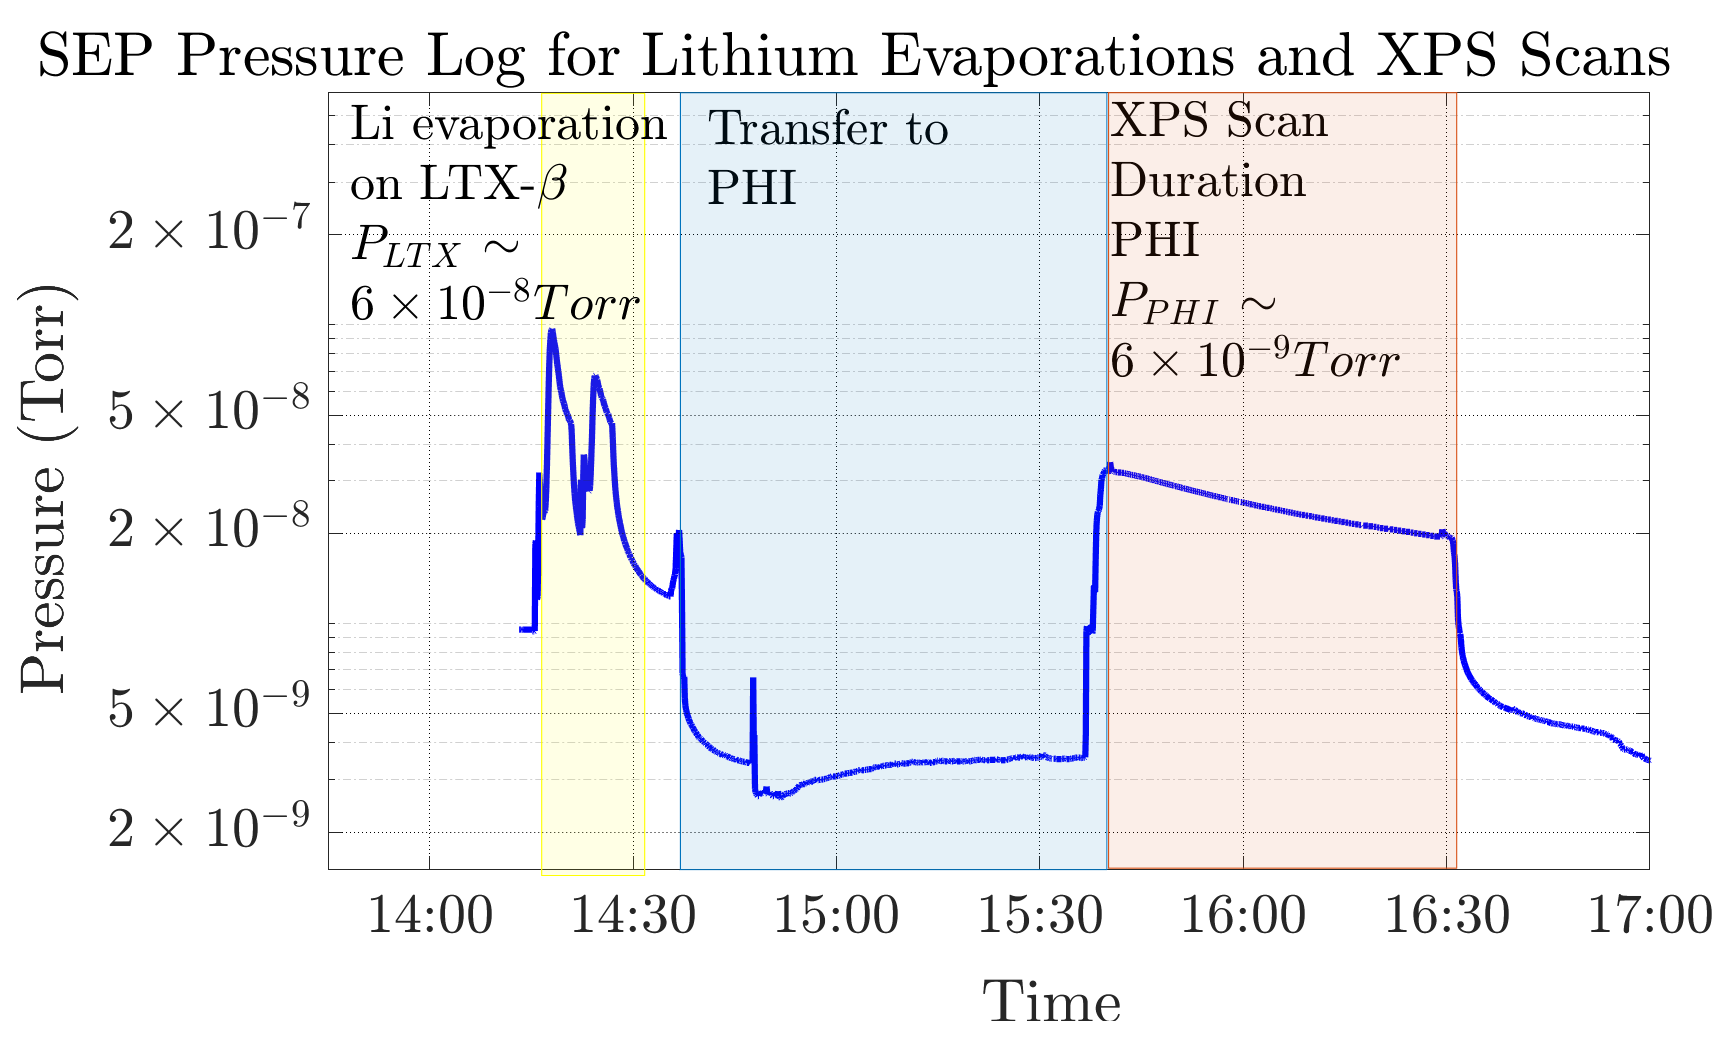
\includegraphics[width=3.37in,keepaspectratio]{04012019_Transferlog}%
\caption{Pressure log from the SEP Ion gauge for transfer from LTX-$\beta$ to PHI, yellow region shows lithium evaporation on the vessel walls, blue region shows SEP pressure during transfer and yellow region for the duration of XPS scans.}
\end{figure}

Because of the vacuum conditions in LTX-$\beta$, during transfer and in the PHI, it is also possible to probe the surface using XPS at time scales comparable to MAPP. Large error bars at shorter time scales exist in MAPP data because of the time to collect counting statistics to quantify elemental composition. A typical MAPP scan took 45 minutes to take a survey over a braod energy range and a few narrow scans of the elements of choice at under vacuum conditions comparable to LTX. The SEP including transfer to PHI takes 2 hours. However, during transfer and XPS scans, the pressure is maintained between $2-7 \times 10^{-9}$ Torr, as shown in figure 4. This is an order of magnitude lower than the LTX-$\beta$ base pressure. Furthermore, the partial pressures of oxygen carrying impurities ($P_{H_2O},P_{CO_2}$, assuming all of $P_{28}$ is CO, to get an upper bound of oxygen carrying impurities) is measured to be between $0.6-1.5 \times 10^{-9}$ Torr in SEP. The partial pressure $P_{H_2O}$ in the PHI during scans is measured to be $8 \times 10^{-10}$ Torr. Since, partial pressures of oxygen carrying impurities are lower in both PHI and SEP compared to LTX-$\beta$ by factor of 2-4, we expect the monolayer formation time to increase by the same factor. Therefore, we expect the surface changes during the MAPP and SEP measurements to be comparable. This is illustrated by the fact that MAPP measured the elemental composition of freshly deposited Li in LTX to be within 70-80 \%. The SEP with PHI measures the same number at 77.4 $\pm$ 4.4 \%.  

It should be pointed out, however, that systems like MAPP can enable analysis at shorter time scales, if compact equipment with improved resolution can be designed and installed where large changes in magnetic fields are expected. Since, MAPP is remotely controllable, where test cell access is limited during plasma operations, these two solutions are presently complimentary to each other.

\begin{acknowledgments}
This work was supported by US Department of Energy contracts DE-AC05-00OR22725, DE-SC0012890, and DE-AC02-09CH11466.

\end{acknowledgments}

%\nocite{*}
\bibliographystyle{aipnum4-1}
\bibliography{references}% Produces the bibliography via BibTeX.

\end{document}
%
% ****** End of file aipsamp.tex ******